\documentclass[../Head/Main.tex]{subfiles}
\begin{document}
\section{Photogrammetry}
IN THIS SECTION SHOULD BE INCLUDED:
\begin{itemize}
\item Bundle adjustment
\item Digitial elevation model
\item Orthorectification and orthomosaic creation
\item EXIF data
\item Number of images and approximate overlap
\item Size of orthomosaic (resolution and disk size)
\item Description of handling outside the fence data (cropping of the image)
\item Screen shots of DSM and orthomosaic

\subsection{Exif data}
The camera used was a senseFly S.O.D.A. with an image resolution of 5472 z 3648 pixels. The type of UAV was not specified by the EXIF informations but it was either a senseFly eBee X or eBee Classic.


senseFly S.O.D.A.\\
Exposure Time : 1/1000\\
Aperture      : 2.8\\
ISO           : 200
Exposure program : AE (exposure priority)
Focal length  : 10.2 mm
Image size    : 5472 x 3648
White balance : Auto
Pitch                           : 6.029021
Roll                            : -7.621159
Yaw                             : 316.127563



\begin{figure}[H]
	\centering
	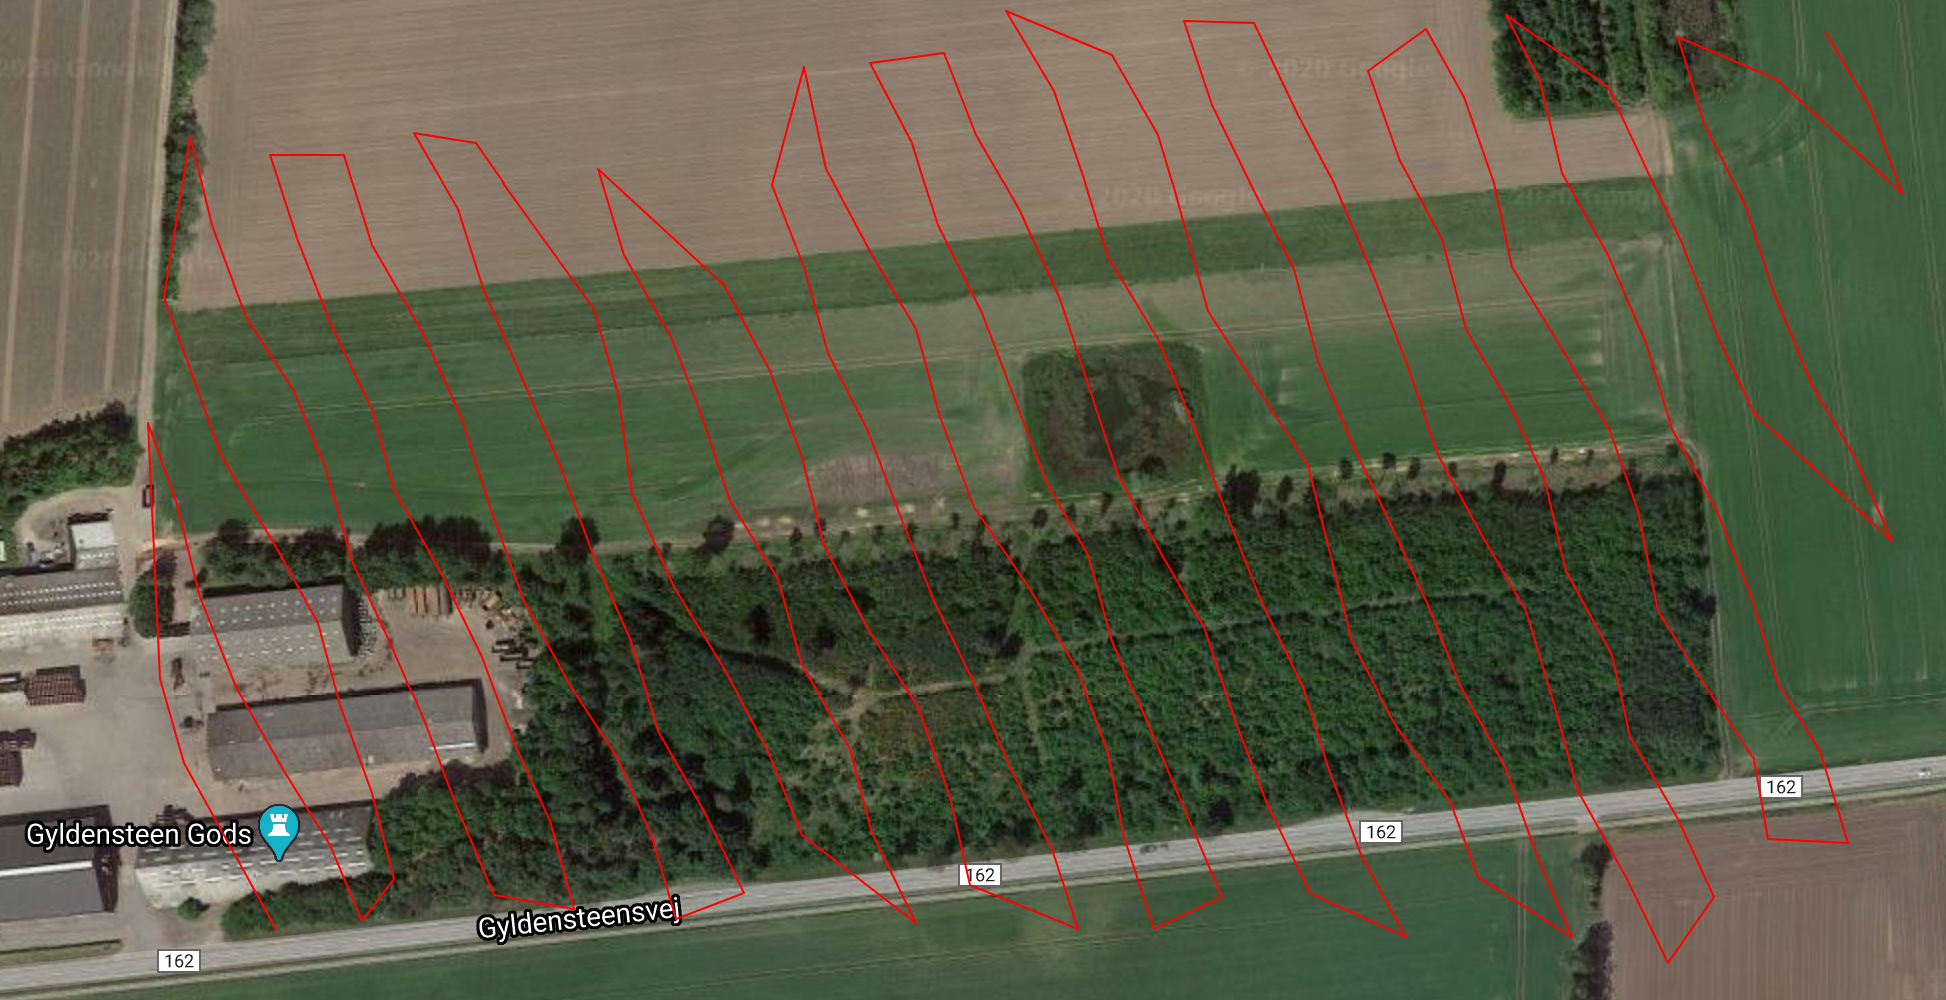
\includegraphics[width=0.75\textwidth]{../Figures/Flight_path}
	\caption{Illustration of the image path}
	\label{fig:flight_path}
\end{figure}

55.56666388888888 10.149922222222221\\
55.569547222222226 10.149922222222221\\
55.569547222222226 10.159333333333334\\
55.56666388888888 10.159333333333334\\

\end{itemize}



\end{document}